\section{Protuberanzen}\label{sec:prominences}
Ein weiterer wesentlicher Bestandteil dieser Arbeit besteht darin, die
Protuberanzen der Sonne, umgangsprachlich Sonnenstürme, zu simulieren. Anders
als bei der Sonnenoberfläche und ihrer Textur wird hier versucht, diese
anhand von physikalischen Eigenschaften der Sonne zu berechnen. Ferner sollen
Magnetfelder berechnet werden, die Einfluss auf Partikel der Sonne nehmen.
Dadurch sollen Protuberanzen entstehen und simuliert werden.

Eine Protuberanz ist ein auf der Sonnenoberfläche auftretendes Phänomen. Sie
entstehen durch abprupte Neuverbindungen von Magnetfeldlinien. Dies wird auch
als Rekonnexion bezeichnet und geschieht immer dann, wenn zwei sich zwei
Magnetfelder aufeinander zu ausbreiten und sich dann neu verbinden
\cite{SpanierReconnexion}. Dabei wird eine große Menge Energie freigesetzt,
die dann Material aus der Sonne hinausschleudert \cite{ZirinProminences}. Da
die Sonne vermutlich nicht nur ein einfaches Magnetfeld besitzt, wäre eine
vollständige Simulation aller Magnetfelder bzw. Pole nicht sinnvoll, da dies
ab einer bestimmten Anzahl von Magnetfeldern einen zu hohen Rechenaufwand
bedeuten würde und man die Phänomenen nicht in Echtzeit darstellen könnte.
Deshalb wird sich im folgenden auf das Modell eines Dipols gestützt, welches
einfach zu berechnen und trotzdem realitätsnahe Ergebnisse erzielen kann. Ein
Dipol ist im Prinzip ein einfacher Magnet und besteht aus zwei
unterschiedlichen Ladungen, anhand dessen ein Magnetfeld berechnet werden
kann. Der Dipol ist das einfachste Modell, welches sich mit Magnetismus
beschäftigt. Die magnetische Flussdichte $\vec{B}$ eines Dipols wird durch
folgende Gleichung beschrieben \cite{Stoecker2013}.
\[
  \vec{B}(\vec{r}) = \frac{\mu_0}{4\pi r^2} \frac{3\vec{r}(\vec{m} \cdot
  \vec{r}) - \vec{m}r^2}{r^3}
\]
Dabei beschreibt $\vec{r}$ den Positionsvektor des zu betrachtenden Punktes
und $r = \vert\vec{r}\vert$ die Länge von $\vec{r}$, $\mu_0$ die magnetische
Feldkonstante und $\vec{m} = p(\vec{r}_+ - \vec{r}_-)$, wobei $p$ die
Polstärke, $\vec{r}_+$ die Position vom Pluspol und $\vec{r}_-$ die Position
vom Minuspol sind \cite{brown1962magnetostatic}. Mithilfe dieser Gleichung
lassen sich für alle Punkte in dem Magnetfeld eines Dipols die entsprechenden
Kräfte berechnen.

\subsection{Vektorenfelder und Partikel}
Das Problem bei der Simulation von Wolken, Rauch, Feuer und auch von
Protuberanzen ist, dass diese Gebilde nicht wohlgeformt sind, wie
beispielsweise ein Würfel, eine Kugel oder sogar ein 3D-Modell eines
Gebäudes. Anstatt zu versuchen Rauch mithilfe von starren Körpern
darzustellen, kam man auf die Idee, Partikelsysteme zu definieren. Partikel
repräsentieren dabei keine einzelnen Objekte, sondern haben die Aufgabe,
Objekte aufgrund ihrer Eigenschaften selbst zu formen. Dabei sind die Partikel
keine statischen Entitäten, sondern üben Kräfte untereinander aus und erfahren
Kräfte von außen, die beispielsweise eine Bewegung der einzelnen Partikel
hervorrufen. Ferner besitzen Partikel bestimmte Eigenschaften wie z.B. eine
Lebensdauer, wodurch sie \textit{geboren} werden, aber auch \textit{sterben}
können. Weitere übliche Eigenschaften sind Geschwindigkeit, Position, Größe,
Farbe und Form. Ein Objekt, welches durch ein Partikelsystem dargestellt
wird, ist nicht deterministisch, da seine Form nicht komplett beschrieben
wird. Stattdessen werden stochastische Methoden angewandt, um das Aussehen
dieser Objekte zu verändern \cite{Reeves1983}.

Auch im Falle der Sonne, um die es in dieser Arbeit handelt, können
Partikelsysteme dabei helfen, komplexe Phänomene realitätsnah darzustellen,
anstatt sie in vorherigen Arbeitsprozessen statisch zu modellieren. In diesem
Projekt werden Partikelsysteme von Unity verwendet. Genauer gesagt werden
\textit{Visual-Effect-Graphen} definiert, welche die Partikel und Kräfte, die
auf sie einwirken, kontrollieren. Damit sollen vor allem versucht werden, die
auf der Sonne auftretenden Protuberanzen zu simulieren. Hierfür wird der im
Abschnitt \ref{sec:prominences} kurz besprochene Dipol verwendet werden. Die
Idee ist, nicht alle Magnetfelder der Sonne abzubilden, Rekonnexionen ihrer
Magnetfeldlinien zu berechnen und damit Protuberanzen zu erzeugen, sondern
pro Protuberanz einen Dipol zu definieren, welcher die Form eines solchen
Materiestroms beeinflusst bzw. hervorruft. Um nun ein Magnetfeld als
Krafteinwirkung auf Partikel zu erstellen, wird ein Vektorenfeld aufgebaut
und anschließend als 3-dimensionale Textur gespeichert. Diese Textur wird
dann in das Partikelsystem eingebaut und beeinflusst damit die Bewegung und
Geschwindigkeit der Partikel.

Ein Vektorfeld ist eine Sammlung von Vektoren, die jeweils eine Position
und eine Richtung besitzen. Damit erfährt jedes Objekt, welches sich an einer
bestimmten Stelle innerhalb des Vektorfeld befindet, eine Kraft in der
jeweiligen Richtung. Um ein solches Feld zu erzeugen,
werden Vektoren gleichmäßig im Raum verteilt. Anschließend werden die Richtungen
mithilfe der magnetischen Flussdichten für jeden dieser Vektoren bestimmt, sodass
sich diese anhand des Magnetfelds ausrichten. Jetzt, wo Vektoren im Raum
verteilt und ihre Richtungen definiert wurden, wird eine 3D-Textur erzeugt, die
all diese Informationen speichert. Dabei wird die Position eines Vektors durch
den Index des Pixels und die Richtung durch eine Farbe innerhalb der Textur
repräsentiert. Abbildung \ref{fig:dipole-vector-field-unity} stellt dies in einem
zweidimensionalen Raum dar. Die damit erstellte 3D-Textur bestehend aus
Richtungsvektoren, die von einer Position abhängen, kann nun innerhalb eines
Partikelsystems verwendet werden. Damit die Partikel die Form einer Protuberanz
annehmen, müssen deren Eigenschaften entsprechend justiert werden. Beispielsweise
muss die initiale Position der Partikel innerhalb der Sonne sein. Dann muss eine
explosionsähnliche Kraft auf sie einwirken, die die Partikel nach außen treibt.
Diese Kraft simuliert damit die Rekonnexion von Magnetfeldlinien und steht senkrecht
auf der Sonnenoberfläche und zeigt nach außen. Da das Magnetfeld ebenfalls vorhanden
ist, werden sich die Partikel entlang der Magnetfeldlinien bewegen. Das Ergebnis
sind Protuberanzen, die mithilfe eines Dipols simuliert und in Abbildung \ref{fig:flare}
betrachtet werden können.

\begin{figure}
  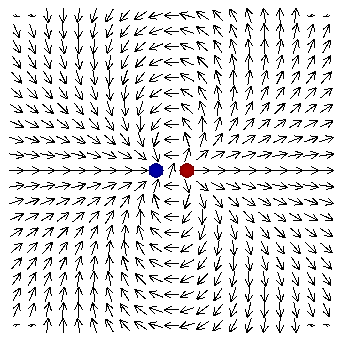
\includegraphics[width=0.75\columnwidth]{dipole-vector-field-unity}
  \caption{In Unity berechnete Magnetfeldlinien des Dipol-Modells. Der Einfachheit halber wird hier ein 2D-Vektorenfeld dargestellt.}
  \label{fig:dipole-vector-field-unity}
  \Description[Dipole]{Magnetfeldlinien eines Dipols.}
\end{figure}

\begin{figure}
  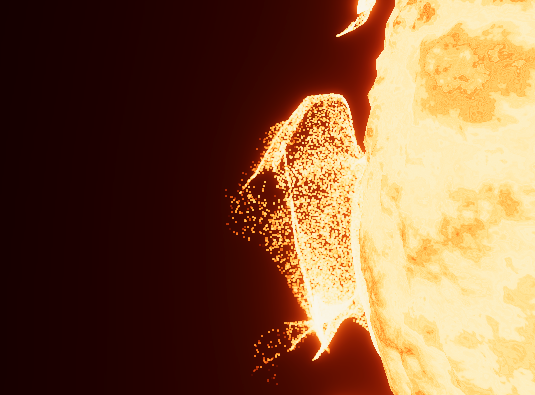
\includegraphics[width=\columnwidth]{flare}
  \caption{Kraftauswirkung eines Dipol-Magnetfeldes auf Partikel der Sonne. Das Ergebnis sind vereinfachte Protuberanzen.}
  \label{fig:flare}
  \Description[Protuberanzen]{Kraftauswirkung eines Dipol-Magnetfeldes auf Partikel der Sonne. Das Ergebnis sind vereinfachte Protuberanzen.}
\end{figure}